\documentclass[10pt]{article}
\usepackage[margin=0.9in]{geometry}
\usepackage{fontspec}
\usepackage{booktabs,graphicx,xcolor,tabularx,amsmath,float,array}
\usepackage[hidelinks]{hyperref}
\setlength{\parskip}{3pt}\setlength{\parindent}{0pt}
\setlength{\abovecaptionskip}{3pt}\setlength{\belowcaptionskip}{2pt}
\setlength{\textfloatsep}{8pt}\setlength{\floatsep}{6pt}\setlength{\intextsep}{6pt}
\renewcommand{\arraystretch}{1.05}
% Long \texttt{} paths and feature names cannot hyphenate; let TeX stretch the
% interword space a little rather than push a line past the margin.
\emergencystretch=3em
\hyphenpenalty=1000
\newcommand{\sig}{$^{*}$}
\newcommand{\fitwidth}[1]{\resizebox{\ifdim\width>\linewidth\linewidth\else\width\fi}{!}{#1}}
\newenvironment{tightitem}{\begin{itemize}\setlength{\itemsep}{1pt}\setlength{\parskip}{0pt}\setlength{\topsep}{2pt}}{\end{itemize}}
\begin{document}
\begin{center}
{\Large\bfseries Design Note --- Assignment 2: Learning from Click-Logs on MIND and EB-NeRD}\\[4pt]
CS4.406 Information Retrieval \& Extraction \quad$\cdot$\quad Parth Dhawale \quad\&\quad Peeyush Prashant\\[2pt]
{\small Code: \url{https://github.com/Zenith053/Assignment1-IRE} (branch \texttt{parth/q4-serving})}
\end{center}
\vspace{-4pt}
\section{What we built}
A two-stage news recommender on MIND-small and EB-NeRD \emph{small} (EB-NeRD was rebuilt from demo to small
for A2, $\sim$10$\times$ more data). \textbf{Stage 1} (A1's candidate generator) retrieves up to 200 candidates
per request: BM25 top-80 $\cup$ FAISS top-100 over A1 embeddings (MiniLM for MIND, the provided word2vec for
EB-NeRD) $\cup$ train-popularity top-20. \textbf{Stage 2} re-ranks them. We built two families of re-rankers:
a GBDT/MLP over hand-crafted behavioural features (Q1--Q2) and NRMS~\cite{nrms}, the official baseline, plus a
popularity/freshness extension (Q3). Every evaluation is on a strict temporal split
(MIND train 2019-11-09 -- 2019-11-12, test 2019-11-15 -- 2019-11-15; EB-NeRD train 2023-05-18 -- 2023-05-23,
test 2023-05-25 -- 2023-06-01); each split's user histories come from a snapshot that ends before the split starts,
asserted by tests (\texttt{tests/test\_no\_leakage.py}). Two evaluation \emph{universes} are kept apart:
\textbf{A} re-ranks the impression's own shown (inview) list, which is what Codabench scores, and
\textbf{B} is the full pipeline: retrieve 200 from the catalogue, then re-rank.
\begin{table}[H]\centering\small
\caption{Data used throughout (temporal splits; the shipped held-out file is the test split).}\label{tab:data}
\fitwidth{\begin{tabular}{lrrrrrr}\toprule
dataset & train imp. & val imp. & test imp. & articles & cand./imp. & test users $<$20 clicks \\\midrule
MIND-small & 95,071 & 61,894 & 73,152 & 65,238 & 23 & 59\% \\
EB-NeRD small & 192,884 & 40,003 & 244,647 & 20,738 & 9 & 16\% \\
\bottomrule\end{tabular}}\end{table}
\section{Q1: Click-history, session and article features}
\begin{table}[H]\centering\small
\caption{Q1 feature table. $^{E}$EB-NeRD only (MIND has no timestamps, sessions or publish times); on MIND these are NaN, never faked.}\label{tab:features}
\fitwidth{\begin{tabular}{lp{0.78\linewidth}}\toprule
group & features (30 in total) \\\midrule
Click history & history length (raw, log), categories, category entropy, decay-weighted mass; hours since last click$^{E}$, mean past dwell time and scroll$^{E}$ \\
Session & candidate position (raw, normalised), inview size, hour of day, day of week; index in session, clicks so far, seconds since session start$^{E}$ \\
Article & train clicks (log), popularity rank, is-head, \textbf{trailing clicks 24 h / 168 h}, title length; \textbf{freshness (hours since publish)}$^{E}$ \\
Match & category match, category match rate; BM25 and semantic score and their in-impression ranks, popularity rank in impression \\
\bottomrule\end{tabular}}\end{table}

\textbf{Behaviour-window boundary.} Two new mechanisms read \emph{other} impressions, so each has its own test:
trailing click counts count only clicks with timestamp strictly before the impression (a counterfactual test
rebuilds the counter from past-only events and demands identical counts), and session features are asserted
strictly increasing in real time. Columns only known after the click (current \texttt{read\_time},
\texttt{scroll\_percentage}, lifetime \texttt{total\_pageviews} \dots) are excluded from every feature; a
user's \emph{past} dwell time is an ordinary feature. The pre-computed \texttt{hybrid} score is excluded
because it was fitted on the validation split that also early-stops the re-rankers.
\section{Q2: Retrieve-then-rank re-rankers}
\textbf{Architecture.} \emph{Option A:} LightGBM with a LambdaRank objective~\cite{lightgbm,lambdamart} (optimises
nDCG directly; 31 leaves, $\ge$30 samples per leaf, L2 1.0, feature fraction 0.7, early stopping on validation
nDCG@10). \emph{Option B:} a small MLP (64--32) trained with a listwise softmax per impression, with a
missing-value indicator per feature so NaN features are usable. Both train on the train split, early-stop on
validation, and report on test. Raw train-click counts were replaced by in-impression ranks after they
dominated the GBDT's splits (a high-cardinality bias) and made it lose to semantic.

\begin{table}[H]\centering\footnotesize
\caption{Q2, Universe A (re-rank the shown list), test metrics on 10,000 impressions per dataset.}\label{tab:q2a}
\fitwidth{\begin{tabular}{lrrrrrr}\toprule
 & MIND AUC & MRR & nDCG@10 & EB AUC & MRR & nDCG@10 \\\midrule
A1 popularity & 0.4955 & 0.2182 & 0.2836 & 0.4441 & 0.2629 & 0.3839 \\
A1 BM25 & 0.5702 & 0.2658 & 0.3445 & 0.5204 & 0.3292 & 0.4450 \\
A1 semantic (before) & 0.6443 & 0.3140 & 0.4033 & 0.5296 & 0.3370 & 0.4538 \\
GBDT (after) & 0.6220 & 0.3013 & 0.3865 & 0.7499 & 0.5226 & 0.6208 \\
MLP (after) & 0.5907 & 0.2796 & 0.3524 & 0.6065 & 0.3684 & 0.4946 \\
\bottomrule\end{tabular}}\end{table}
\begin{table}[H]\centering\footnotesize
\caption{Q2, after vs before (best single A1 scorer, semantic on both): paired bootstrap 95\% CI, 10,000 resamples; $^{*}$ = CI excludes zero. MRR and nDCG@5 move the same way (all significant).}\label{tab:q2d}
\fitwidth{\begin{tabular}{lrrrr}\toprule
 & MIND $\Delta$AUC & MIND $\Delta$nDCG@10 & EB $\Delta$AUC & EB $\Delta$nDCG@10 \\\midrule
GBDT $-$ semantic & $-$0.022 [$-$0.026, $-$0.018]$^{*}$ & $-$0.017 [$-$0.020, $-$0.014]$^{*}$ & +0.220 [+0.213, +0.228]$^{*}$ & +0.167 [+0.160, +0.174]$^{*}$ \\
MLP $-$ semantic & $-$0.054 [$-$0.061, $-$0.046]$^{*}$ & $-$0.051 [$-$0.057, $-$0.045]$^{*}$ & +0.077 [+0.069, +0.085]$^{*}$ & +0.041 [+0.034, +0.047]$^{*}$ \\
\bottomrule\end{tabular}}\end{table}
\begin{table}[H]\centering\footnotesize
\caption{Q2, Universe B (retrieve top-200, then re-rank), 3,000 test impressions each. Accuracy is conditional on a click being retrieved; end-to-end = recall $\times$ conditional.}\label{tab:q2b}
\fitwidth{\begin{tabular}{lrr}\toprule
 & MIND & EB-NeRD small \\\midrule
recall@200 (click retrieved) & 0.235 & 0.096 \\
AUC | retrieved, stage-1 order & 0.673 [0.657, 0.689] & 0.444 [0.413, 0.479] \\
AUC | retrieved, GBDT & 0.494 [0.477, 0.512] & 0.917 [0.896, 0.935] \\
nDCG@10 | retrieved, before $\to$ after & 0.060 $\to$ 0.012 & 0.017 $\to$ 0.409 \\
end-to-end nDCG@10, before $\to$ after & 0.0141 $\to$ 0.0029 & 0.0016 $\to$ 0.0393 \\
\bottomrule\end{tabular}}\end{table}

\textbf{Observations.} Re-ranking over behavioural features \emph{loses} to A1's semantic scorer on MIND
(significant on every metric) but \emph{wins} by $+0.22$ AUC on EB-NeRD. Top GBDT features (gain):
MIND \texttt{train\_clicks\_log1p} 0.19, \texttt{semantic} 0.15, \texttt{popularity\_rank} 0.10; EB-NeRD \texttt{rolling\_clicks\_24h} 0.27, \texttt{freshness\_hours} 0.13, \texttt{rolling\_clicks\_168h} 0.09. EB-NeRD is driven by \emph{what is being clicked now} and
\emph{how new the article is} --- the signals Q3 adds to NRMS. Stage 1 caps the whole system: 76\% (MIND) and
90\% (EB-NeRD) of test clicks are never retrieved. On retrieved lists the GBDT trained on shown negatives is at
chance on MIND (the negatives' distribution shifts) but near-perfect on EB-NeRD, where freshness and trailing
clicks separate the one live article from mostly stale retrieved ones. Making Q2 run required pinning LightGBM
and FAISS to one thread (faiss, torch and LightGBM each link an incompatible OpenMP runtime; multi-threaded
training segfaulted), and fixing a metric bug that had applied recall twice in Universe B.
\section{Q3: Baseline reproduced, then beaten}
\textbf{Baseline: NRMS}~\cite{nrms}, the official ebnerd-benchmark baseline, ported to PyTorch with the
benchmark's hyperparameters: title length 30, history 20, 4 sampled negatives per click, 20 heads $\times$ 20
dims, additive attention 200, dropout 0.2, Adam $10^{-4}$, batch 32, trainable word embeddings initialised from
XLM-RoBERTa-base~\cite{xlmr} (one multilingual vocabulary for Danish and English). A news encoder (multi-head
self-attention over title tokens, additive pooling) and a user encoder (the same over the last 20 clicked
articles) give 400-d vectors; the score is their dot product. Deviations: PyTorch port; padding masked out of
every softmax (59\% of MIND test users have $<$20 clicks); evaluated on our temporal split, so numbers are not
the published ones. NRMS is \emph{below} A1 semantic on MIND ($\Delta$AUC $-$0.0186 [$-$0.0209, $-$0.0164]$^{*}$) and \emph{above} it
on EB-NeRD (+0.0236 [+0.0218, +0.0253]$^{*}$), where A1 only had the weaker provided word2vec vectors.

\textbf{Principled change: popularity- and freshness-aware NRMS} (after PP-Rec~\cite{pprec}). NRMS reads only
titles, but news decays within hours and Q2 showed trailing clicks and article age are EB-NeRD's strongest
signals. Each candidate gets $\log(1+\cdot)$ of its clicks in the trailing 1\,h / 24\,h / 7\,d (strictly before the
impression; the vectorised counter is tested equal to Q1's causal \texttt{RollingPopularity}) and, on EB-NeRD, its
age. A small MLP turns them into a signal score, blended with the content score by a per-user gate
$g=\sigma(w^\top u+b)$: $s=(1-g)\,s_\text{content}+g\,s_\text{signal}$; the ablation replaces the gate with a plain
sum. The variant reported as ``improved'' is chosen by mean \emph{validation} AUC among pre-stated candidates
(MIND: plain sum 0.6348 vs gate 0.6317), never by test.

\begin{table}[H]\centering\footnotesize
\caption{Q3 baseline vs improved on the full test splits, 3 seeds each (MRR and nDCG are seed means).}\label{tab:q3main}
\fitwidth{\begin{tabular}{llcrrrr}\toprule
 & model & test AUC, seeds 13 / 14 / 15 & AUC mean $\pm$ sd & MRR & nDCG@5 & nDCG@10 \\\midrule
MIND-small & NRMS (baseline) & 0.6232 / 0.6217 / 0.6261 & 0.6237 $\pm$ 0.0022 & 0.2959 & 0.3214 & 0.3835 \\
 & improved: \texttt{nrms\_pop\_sum} & 0.6359 / 0.6190 / 0.6314 & 0.6288 $\pm$ 0.0088 & 0.2972 & 0.3236 & 0.3860 \\
EB-NeRD small & NRMS (baseline) & 0.5539 / 0.5488 / 0.5498 & 0.5508 $\pm$ 0.0027 & 0.3471 & 0.3865 & 0.4645 \\
 & improved: \texttt{nrms\_popfresh} & 0.7246 / 0.7257 / 0.7265 & 0.7256 $\pm$ 0.0010 & 0.4860 & 0.5486 & 0.5928 \\
\bottomrule\end{tabular}}\end{table}
\begin{table}[H]\centering\footnotesize
\caption{Q3 significance: paired bootstrap 95\% CI (10,000 resamples) on each test impression's metric averaged over the 3 seeds; $^{*}$ = CI excludes zero.}\label{tab:q3ci}
\fitwidth{\begin{tabular}{lrrrr}\toprule
improved $-$ NRMS & $\Delta$AUC & $\Delta$MRR & $\Delta$nDCG@5 & $\Delta$nDCG@10 \\\midrule
MIND-small & +0.0051 [+0.0043, +0.0060]$^{*}$ & +0.0013 [+0.0004, +0.0021]$^{*}$ & +0.0022 [+0.0013, +0.0032]$^{*}$ & +0.0025 [+0.0016, +0.0034]$^{*}$ \\
EB-NeRD small & +0.1748 [+0.1733, +0.1761]$^{*}$ & +0.1389 [+0.1375, +0.1404]$^{*}$ & +0.1622 [+0.1607, +0.1636]$^{*}$ & +0.1283 [+0.1270, +0.1295]$^{*}$ \\
\bottomrule\end{tabular}}\end{table}

\begin{table}[H]\centering\footnotesize
\caption{Q3 ablation, paired bootstrap 95\% CI on the full test split; $^{*}$ = CI excludes zero.}\label{tab:q3abl}
\fitwidth{\begin{tabular}{lrrr}\toprule
ablation (EB-NeRD: seed 13) & $\Delta$AUC & $\Delta$MRR & $\Delta$nDCG@10 \\\midrule
EB-NeRD: + freshness only vs NRMS & +0.093 [+0.092, +0.094]$^{*}$ & +0.072 [+0.070, +0.073]$^{*}$ & +0.068 [+0.066, +0.069]$^{*}$ \\
EB-NeRD: + popularity only vs NRMS & +0.171 [+0.169, +0.172]$^{*}$ & +0.135 [+0.134, +0.137]$^{*}$ & +0.125 [+0.123, +0.126]$^{*}$ \\
EB-NeRD: + both, learned gate (full) vs NRMS & +0.171 [+0.169, +0.172]$^{*}$ & +0.138 [+0.137, +0.140]$^{*}$ & +0.127 [+0.126, +0.128]$^{*}$ \\
EB-NeRD: + both, plain sum vs NRMS & +0.170 [+0.168, +0.171]$^{*}$ & +0.138 [+0.137, +0.140]$^{*}$ & +0.127 [+0.126, +0.129]$^{*}$ \\
EB-NeRD: popularity only vs full & +0.000 [$-$0.000, +0.001] & $-$0.003 [$-$0.004, $-$0.002]$^{*}$ & $-$0.003 [$-$0.003, $-$0.002]$^{*}$ \\
EB-NeRD: freshness only vs full & $-$0.078 [$-$0.079, $-$0.077]$^{*}$ & $-$0.066 [$-$0.068, $-$0.065]$^{*}$ & $-$0.060 [$-$0.061, $-$0.059]$^{*}$ \\
EB-NeRD: plain sum vs learned gate & $-$0.001 [$-$0.002, $-$0.001]$^{*}$ & +0.000 [$-$0.000, +0.001] & +0.000 [$-$0.000, +0.001] \\
MIND: + popularity, learned gate vs NRMS (seed 13) & +0.005 [+0.004, +0.006]$^{*}$ & +0.000 [$-$0.001, +0.001] & +0.001 [+0.000, +0.002]$^{*}$ \\
MIND: plain sum vs learned gate (3 seeds) & +0.003 [+0.002, +0.003]$^{*}$ & +0.002 [+0.001, +0.002]$^{*}$ & +0.001 [+0.001, +0.002]$^{*}$ \\
\bottomrule\end{tabular}}\end{table}

\textbf{Findings.} (1) On EB-NeRD the change is large and robust: $+0.175$ AUC, significant on every seed and
metric, seed spread $\pm0.001$. Popularity carries almost all of it; freshness alone adds $+0.09$ but is largely
redundant with popularity (no AUC gain on top of it, $+0.003$ MRR/nDCG). (2) Freshness is not monotone: click
rate peaks at 2-4h (0.120) and falls to 0.013 for
articles older than 30 days; ``newer ranks higher'' scores 0.501 AUC,
the bump rule 0.663. (3) The per-user gate does not earn its keep: equal to a plain sum
on EB-NeRD and slightly worse on MIND. (4) On MIND the gain is small ($+0.005$) and \emph{not robust to training
randomness}: seed 14 is significantly worse than its baseline, the seed spread ($\pm0.009$) exceeds the gain, and
validation disagreed with test on that seed. The paired CI covers test-impression sampling, not training noise.
\section{Q5: Extended evaluation}
\begin{table}[H]\centering\scriptsize
\caption{Q5, full two-stage pipeline (Universe B, 3,500 test impressions per dataset), all metrics. Accuracy is conditional on a retrieved click; diversity, novelty (bits) and coverage are over the top-10 shown.}\label{tab:q5}
\fitwidth{\begin{tabular}{llrrrrrrrr}\toprule
 & system & recall & AUC$|$ret. & MRR$|$ret. & nDCG@5$|$ret. & nDCG@10$|$ret. & diversity & novelty & coverage \\\midrule
MIND & stage-1 order & 0.274 & 0.670 [0.655, 0.683] & 0.070 & 0.055 & 0.072 [0.060, 0.085] & 0.682 & 15.70 & 0.029 \\
 & two-stage GBDT & 0.274 & 0.570 [0.556, 0.584] & 0.032 & 0.015 & 0.022 [0.015, 0.029] & 0.852 & 10.04 & 0.017 \\
EB-NeRD & stage-1 order & 0.127 & 0.493 [0.467, 0.520] & 0.035 & 0.018 & 0.032 [0.020, 0.044] & 0.116 & 11.99 & 0.073 \\
 & two-stage GBDT & 0.127 & 0.845 [0.826, 0.863] & 0.217 & 0.215 & 0.258 [0.230, 0.289] & 0.136 & 12.28 & 0.076 \\
\bottomrule\end{tabular}}\end{table}
\begin{table}[H]\centering\scriptsize
\caption{Q5 slices for the two-stage GBDT pipeline, with bootstrap 95\% CIs. EB-NeRD has no cold users under the $<$5-click rule (every user has $\ge$5), so the lowest-history quartile stands in.}\label{tab:q5slices}
\fitwidth{\begin{tabular}{llrrrrr}\toprule
 & slice & n & recall@200 & AUC$|$retrieved & nDCG@10$|$retrieved & diversity \\\midrule
MIND & cold ($<$5 clicks) & 377 & 0.199 & 0.521 [0.461, 0.574] & 0.013 [0.000, 0.029] & 0.880 \\
 & warm & 3,123 & 0.283 & 0.575 [0.558, 0.590] & 0.023 [0.016, 0.030] & 0.849 \\
 & lowest-history quartile & 637 & 0.204 & 0.510 [0.468, 0.548] & 0.014 [0.002, 0.027] & 0.879 \\
 & other users & 2,863 & 0.290 & 0.580 [0.564, 0.595] & 0.023 [0.016, 0.031] & 0.846 \\
 & head click & 100 & 0.500 & 0.728 [0.660, 0.793] & 0.187 [0.103, 0.279] & 0.849 \\
 & tail click & 3,400 & 0.268 & 0.562 [0.548, 0.578] & 0.013 [0.008, 0.018] & 0.853 \\
EB-NeRD & cold ($<$5 clicks) & 0 & -- & -- & -- & -- \\
 & warm & 3,500 & 0.127 & 0.845 [0.826, 0.863] & 0.258 [0.230, 0.289] & 0.136 \\
 & lowest-history quartile & 295 & 0.112 & 0.786 [0.701, 0.861] & 0.235 [0.112, 0.370] & 0.136 \\
 & other users & 3,205 & 0.129 & 0.850 [0.830, 0.866] & 0.260 [0.229, 0.293] & 0.136 \\
 & head click & 17 & 0.882 & 0.920 [0.857, 0.971] & 0.356 [0.194, 0.530] & 0.125 \\
 & tail click & 3,483 & 0.124 & 0.843 [0.825, 0.861] & 0.255 [0.226, 0.290] & 0.136 \\
\bottomrule\end{tabular}}\end{table}

\textbf{Observations.} Beyond-accuracy metrics move against accuracy. On MIND the two-stage GBDT recommends a
\emph{more} diverse but far \emph{less} novel list than stage 1 alone (it learned to push popular articles), and
covers fewer articles; on EB-NeRD it gains accuracy with little change in diversity. Head-click impressions retrieve
far better than tail ones (MIND 0.500 vs 0.268, EB-NeRD 0.882 vs 0.124): much of stage 1's recall comes from the
popularity arm. Lowest-history users retrieve and rank worse on both datasets. Coverage is reported as a point
estimate; head-click slices have 100 (MIND) and 17 (EB-NeRD) impressions, so their CIs are wide.

\textbf{Codabench.} The hidden test sets carry no clicks, so trailing click counts cannot be computed on them. We
measured what that does on our labelled EB-NeRD test split: the best Q3 model scores 0.7246
with real trailing clicks, 0.4810 when counts can only use clicks from before
the test period (only 3.3\% of candidates keep a
non-zero 24\,h count) and 0.4854 with none --- below chance. We therefore submitted the best models
that need no click logs: NRMS on MIND and NRMS + freshness (publish times are in the test files) on EB-NeRD. The
inference path was verified before submitting: on \texttt{MINDsmall\_dev} it reproduces the offline AUC (0.6232;
Microsoft's official \texttt{evaluate.py} gives 0.6235 on the written ranks, the difference being rank ties), and on
EB-NeRD small validation 0.5539 / 0.6459; unseen title tokens use pretrained XLM-R vectors (2.9\% of MIND and 15.8\%
of EB-NeRD test titles), and every zip is validated line by line against the source file (row order, ids, rank
permutations). Rank-averaging click-free scorers looks promising offline (MIND NRMS + A1 semantic
0.6531; EB-NeRD NRMS + freshness with exposure counts
0.6609) but was not submitted.

\textbf{Leaderboard outcome.} Both scored close to what our own splits predicted --- MIND
0.6208 against 0.6232 offline, EB-NeRD 0.6411 against
0.6459 --- so the estimate held on hidden sets of 2,370,727 and 13,536,710
impressions, and the popularity model we did not submit would have scored near chance. EB-NeRD scores 50\% of its
testset and publishes per-day metrics: AUC runs 0.6288--0.6566 over
eight days (day mean 0.6404 vs 0.6411 pooled), so one leaderboard
figure hides $\pm$0.014 of day-to-day movement --- more
than separates most models in Table~\ref{tab:q3main}.
\begin{table}[H]\centering\footnotesize\caption{Codabench submissions (hidden test sets).}\label{tab:cb}
\fitwidth{\begin{tabular}{llrrrrrrr}\toprule
 competition & model & impressions & zip MB & offline AUC & AUC & MRR & nDCG@5 & nDCG@10\\\midrule
MIND 13967 & NRMS & 2,370,727 & 107.3 & 0.6232 & 0.6208 & 0.2904 & 0.3118 & 0.3683\\
EB-NeRD 2469 & NRMS + freshness & 13,536,710 & 221.4 & 0.6459 & 0.6411 & 0.4131 & 0.4689 & 0.5294\\
\bottomrule\end{tabular}}\end{table}
\begin{figure}[H]\centering
\begin{minipage}{0.49\linewidth}\centering 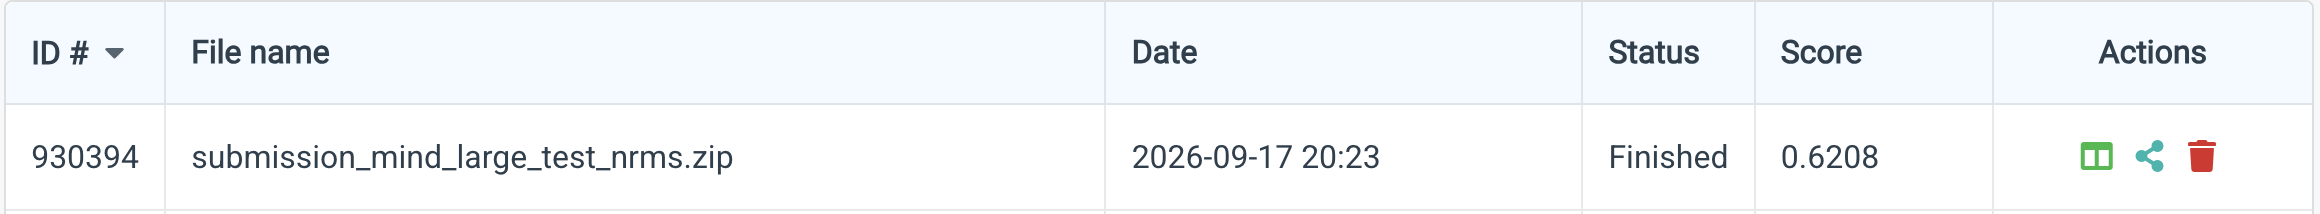
\includegraphics[width=1.0\linewidth,height=1.1cm,keepaspectratio]{screenshots/mind_submission.png}\end{minipage}\hfill
\begin{minipage}{0.49\linewidth}\centering 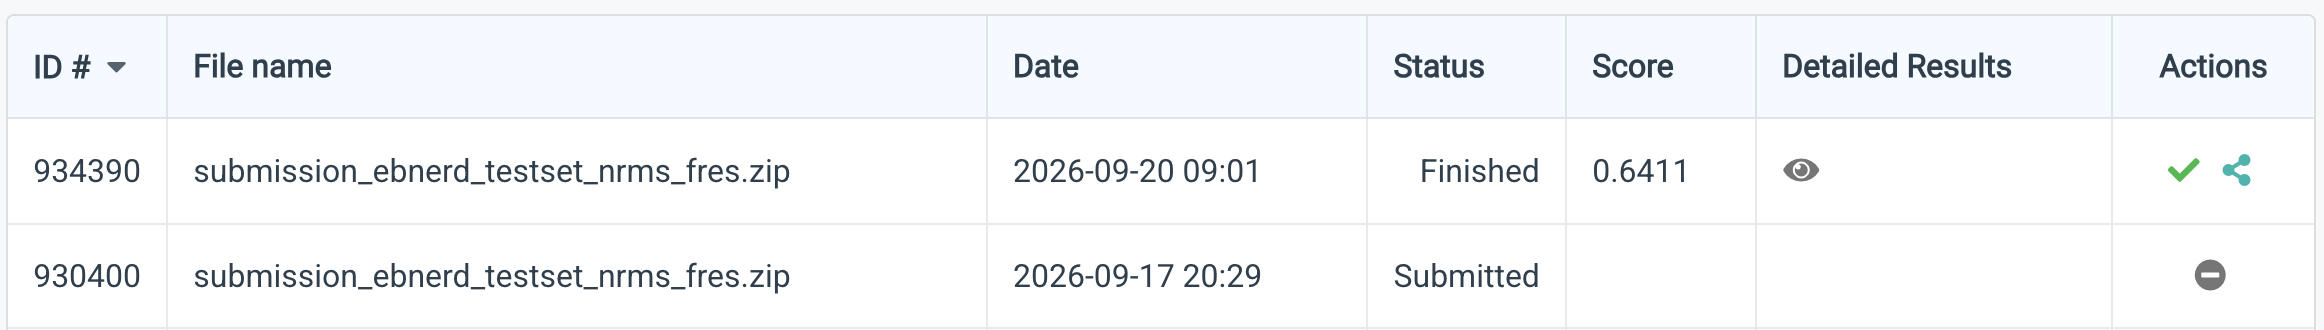
\includegraphics[width=1.0\linewidth,height=1.1cm,keepaspectratio]{screenshots/ebnerd_submission.png}\end{minipage}\\[4pt]

\includegraphics[width=1.0\linewidth,height=0.8cm,keepaspectratio]{screenshots/mind_leaderboard.png}\\[3pt]
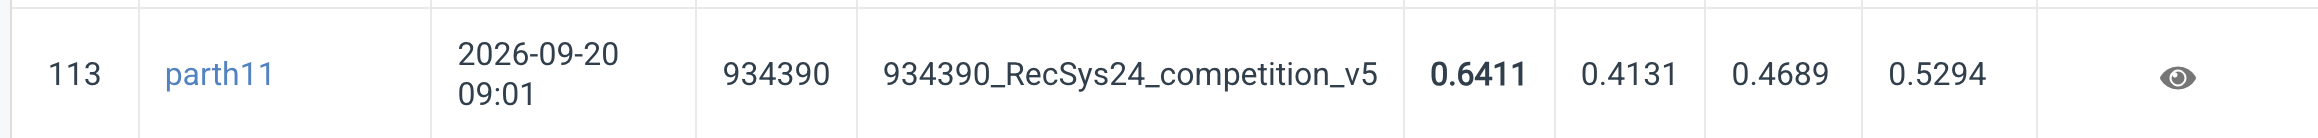
\includegraphics[width=1.0\linewidth,height=1.1cm,keepaspectratio]{screenshots/ebnerd_leaderboard.png}
\caption{Codabench. Top: the two submissions accepted (MIND left, EB-NeRD right). Bottom: our leaderboard rows, MIND above EB-NeRD.}\label{fig:cb}\end{figure}
\section{Q4: Serving and scale analysis}
A one-request serving path loads everything once (indexes, model, every article's NRMS vector, so a request never
encodes text) and times eight stages; it reproduces the offline test scores (max difference
1e-06 MIND, 4e-06 EB-NeRD). PyTorch, FAISS and BLAS
are pinned to one thread (they defaulted to 4--10), so figures are per core.
\begin{table}[H]\centering\footnotesize
\caption{Q4 serving: full two-stage pipeline, one request at a time, Apple M4 CPU, one thread; 2,000 replayed test requests.}\label{tab:q4}
\fitwidth{\begin{tabular}{lrr}\toprule
 & MIND & EB-NeRD small \\\midrule
memory to serve (MB) & 446 & 169 \\
\quad largest: A1 / NRMS article vectors, NRMS weights (MB) & 100 / 104 / 68 & 25 / 33 / 44 \\
ANN index, catalogue: exact FAISS $\to$ HNSW (MB) & 100 $\to$ 118 & 25 $\to$ 31 \\
latency p50 / p95 / p99, one request (ms) & 1.14 / 1.77 / 2.24 & 1.74 / 3.34 / 3.81 \\
\quad same, calling batch code per request (ms) & 26.1 / 28.5 / 29.6 & 9.6 / 11.1 / 11.7 \\
cores at 1k / 10k QPS (sim.\ p99 ms) & 3 / 21 (2.2) & 4 / 32 (3.8) \\
cost per 1,000 queries at 1k QPS & \$0.000033 & \$0.000044 \\
\bottomrule\end{tabular}}\end{table}

\textbf{Findings.} BM25 is the largest stage and sets the tail: its query is the user's whole click history
(EB-NeRD users with 200+ clicks: p99 3.96\,ms vs
1.06\,ms for 1--10). NRMS re-ranking is a constant
$\sim$0.3\,ms: 200 dot products over precomputed vectors. Calling A1's batch
functions per request is 23.0$\times$ slower on MIND, almost all of it
rebuilding an article$\to$tokens dictionary over the whole catalogue per call; caching request-independent work
removes it. \textbf{Cost} (assumed \$0.04/core-hour, one single-threaded worker per core,
60\% utilisation): a queueing simulation driven by the measured request times
(validated against M/M/1 theory) keeps p99 under 10\,ms
even at 95\% utilisation, so the 100\,ms SLA never binds and cost is linear in traffic; a 3$\times$ slower cloud vCPU
still meets it. Network, parsing and remote stores are not in these timings.
\section{Where the system breaks at 10\texorpdfstring{$\times$}{x}}
Measured on a synthetic 10$\times$ catalogue (every article copied 10$\times$ with perturbed vectors; MIND
65,238 $\to$ 652,380 articles) and 10$\times$ click events, replaying 1,000 real users:
\begin{tightitem}
\item \textbf{First: per-request code that touches the whole catalogue.} Calling the batch code per request, MIND p99
goes from 28 to \textbf{308\,ms} and breaks the SLA on a
single request (EB-NeRD 91\,ms). With request-independent work cached,
serving p99 grows only 1.8 $\to$ 4.9\,ms.
\item \textbf{Second: RAM per worker.} Served memory grows 446 $\to$
3,844\,MB; each MIND worker needs 4.2\,GB, above an assumed
4\,GB per vCPU, so RAM, not CPU, sets the bill (60 vCPUs for
57 cores of work at 10$\times$ catalogue and traffic). Fix: share read-only vectors across workers
(memory-mapping) or move them to a vector-search service.
\item \textbf{Third: approximate-search quality.} Exact search over the whole MIND catalogue reaches
18\,ms p99 at 10$\times$, pushing a larger site to HNSW~\cite{hnsw,faiss}, whose
recall@100 falls from 0.81 to 0.46 (efSearch 64; 0.73 at 256). Searching only the
circulating pool avoids this today (1.4\,ms) but the pool grows with the site.
\item \textbf{Not the bottleneck:} stage-2 re-ranking and click-count lookups stay flat; 10$\times$ traffic alone is linear
cost (lower p99 from larger worker pools). Argued, not measured: 10$\times$ click events need a streaming counter, and
the popularity model's accuracy depends on that counter being real-time (it collapses to chance without it, \S5).
\end{tightitem}
Caveats: laptop CPU (indicative per-core numbers); synthetic near-duplicate copies make HNSW recall pessimistic and do
not grow BM25's vocabulary; users $\times$10 is a linear memory extrapolation.
\section{Anti-gaming, limitations and alternatives}
\textbf{Features unavailable at serving time} (Q9). EB-NeRD ships lifetime totals
(\texttt{total\_inviews}, \texttt{total\_pageviews}, \texttt{total\_read\_time}), known only after the fact. Adding them to the A2 GBDT's features inflates every metric significantly (Table~\ref{tab:q9});
using \texttt{total\_pageviews} alone as a popularity score inflates A1's popularity scorer far more,
0.5978 against 0.4459 AUC (+0.1520). The A2 feature table
excludes all of them by default (asserted by \texttt{tests/test\_no\_leakage.py}), and every trailing count is
strictly causal. The Codabench analysis (\S5) is the serving-time version of the same lesson: a feature that is
honest offline can still be unavailable at serving time if the live system does not log it.
\begin{table}[H]\centering\footnotesize
\caption{Q9 on the A2 re-ranker (EB-NeRD small, 10,000 test impressions): the same GBDT trained with the dataset's serving-time-unavailable article totals added. $^{*}$ = CI excludes zero.}\label{tab:q9}
\fitwidth{\begin{tabular}{lrrr}\toprule
metric & honest (A2 features) & with leaked features & inflation, 95\% CI \\\midrule
auc & 0.7499 & 0.7605 & +0.0105 [+0.0074, +0.0136]$^{*}$ \\
mrr & 0.5226 & 0.5315 & +0.0089 [+0.0038, +0.0141]$^{*}$ \\
ndcg@5 & 0.5831 & 0.5954 & +0.0123 [+0.0077, +0.0169]$^{*}$ \\
ndcg@10 & 0.6208 & 0.6288 & +0.0080 [+0.0040, +0.0121]$^{*}$ \\
\bottomrule\end{tabular}}\end{table}


\textbf{Limitations.} MIND's gain is within seed noise; Q3 runs mix Apple-GPU and CUDA hardware across seeds; the
circulating candidate pool is built from the whole test period (slightly optimistic recall); Universe B labels a retrieved
but never-shown article as a non-click; Q5 uses 3,500 impressions and reports coverage without a CI.

\textbf{Alternatives considered.} A cross-encoder or full transformer news encoder (too slow to train on a laptop in the
time available; NRMS epochs took 11--13 min on an M4); retraining the GBDT on retrieved rather than shown negatives
(would fix the MIND distribution shift in Universe B); exposure counts as a click-free popularity proxy for Codabench
(0.636 AUC alone on EB-NeRD, measured but not submitted); HNSW with larger efSearch for a bigger catalogue.
\begin{thebibliography}{9}\small\setlength{\itemsep}{0pt}
\bibitem{nrms} C.~Wu, F.~Wu, S.~Ge, T.~Qi, Y.~Huang, X.~Xie. Neural news recommendation with multi-head self-attention. EMNLP-IJCNLP 2019.
\bibitem{pprec} T.~Qi, F.~Wu, C.~Wu, Y.~Huang. PP-Rec: News recommendation with personalized user interest and time-aware news popularity. ACL 2021.
\bibitem{mind} F.~Wu et al. MIND: A large-scale dataset for news recommendation. ACL 2020.
\bibitem{ebnerd} J.~Kruse et al. EB-NeRD: A large-scale dataset for news recommendation. RecSys Challenge 2024.
\bibitem{xlmr} A.~Conneau et al. Unsupervised cross-lingual representation learning at scale. ACL 2020.
\bibitem{lightgbm} G.~Ke et al. LightGBM: A highly efficient gradient boosting decision tree. NeurIPS 2017.
\bibitem{lambdamart} C.~J.~C.~Burges. From RankNet to LambdaRank to LambdaMART: An overview. Microsoft Research TR 2010.
\bibitem{hnsw} Y.~A.~Malkov, D.~A.~Yashunin. Efficient and robust approximate nearest neighbor search using HNSW graphs. TPAMI 2020.
\bibitem{faiss} J.~Johnson, M.~Douze, H.~J\'egou. Billion-scale similarity search with GPUs. IEEE Trans.\ Big Data 2021.
\end{thebibliography}
\appendix
\section{Reproduce}
{\small\begin{verbatim}
make data                       # A1 pipeline; EB-NeRD rebuilt at scale: small
make q1 q2 q3 q4 q5 q6          # one target per question, in order
\end{verbatim}}
\vspace{-6pt}
Codabench zips come from \texttt{src/submission/predict\_nrms.py} and are checked by
\texttt{validate\_zip.py}. Detailed tables are in \texttt{reports/q3\_summary.md} and
\texttt{reports/q4\_summary.md}; per-question implementation notes in \texttt{reports/a2\_q*\_implementation.md};
AI assistance in \texttt{reports/a2\_ai\_usage\_log.md} (A1's in \texttt{reports/ai\_usage\_log.md}); the run logs
behind every number in \texttt{logs/}. The build also writes three figures to
\texttt{reports/design\_note/figures/}, omitted here for length.
\end{document}
